\documentclass{beamer}

% ================= Packages =================
\usepackage{hyperref}
\usepackage[T1]{fontenc}
\usepackage[utf8]{inputenc}

% Math, figures, tables
\usepackage{latexsym,amsmath,xcolor,multicol,booktabs,array}
\usepackage{graphicx,listings,stackengine}

% Bibliography package kept for compatibility with the theme/source tree.
\usepackage{natbib}
\bibliographystyle{plainnat}

% ================= CUHKSZ Theme =================
\usepackage{CUHKSZ}
\setbeamertemplate{headline}{}

% ================= Color & Code Style =================
\def\cmd#1{\texttt{\color{red}\footnotesize $\backslash$#1}}
\def\env#1{\texttt{\color{blue}\footnotesize #1}}

\xdefinecolor{cuhksz1}{rgb}{0.457,0.0585,0.42578}
\xdefinecolor{cuhksz2}{rgb}{0.86328,0.63671875,0}
\xdefinecolor{cuhksz3}{rgb}{0.953125,0.87109,0.6875}
\definecolor{deepred}{rgb}{0.6,0,0}

\lstset{
    basicstyle=\ttfamily\small,
    keywordstyle=\bfseries\color{cuhksz1},
    emphstyle=\ttfamily\color{deepred},
    stringstyle=\color{cuhksz2},
    numbers=left,
    numberstyle=\small\color{cuhksz3},
    frame=shadowbox,
}

\newcommand{\metric}[1]{\textsc{#1}}
\newcommand{\setting}[1]{\textbf{#1}}
\newcommand{\takeaway}[1]{\begin{block}{Takeaway}#1\end{block}}

% ================= Title Information =================
\title[Low-Data RLVR Calibration]{Behavioral Calibration for Mathematical Reasoning under Low-Data Reinforcement Learning}
\subtitle{Controlled Experiments and Token-Level Evidence for 1-shot GRPO}
\author[Zihang Xu]{Zihang Xu}
\institute[CUHK-Shenzhen]{Data Science, The Chinese University of Hong Kong, Shenzhen}
\date{Capstone Project Final Presentation}

% ================= Document =================
\begin{document}

% 1
\begin{frame}
\titlepage
\end{frame}

% 2
\begin{frame}{Three Questions}
\begin{block}{Central Goal}
Explain whether 1-shot GRPO produces a real held-out gain, where that gain comes from, and what mechanism best explains it.
\end{block}

\begin{enumerate}
    \item \textbf{Does it help?} Does 1-shot GRPO improve MATH500 accuracy beyond the initial model?
    \item \textbf{Where does the gain come from?} Is it tied to reward semantics, data budget, group-relative signal, or model family?
    \item \textbf{What is the mechanism?} Does training create new knowledge, or calibrate how existing reasoning behavior is expressed?
\end{enumerate}

\takeaway{The evidence supports a calibration account: 1-shot GRPO helps the Base model when the reward is meaningful, mainly by stabilizing the generation distribution.}
\end{frame}

% 3
\begin{frame}[shrink=5]{Evidence Design}
\begin{columns}
\column{0.48\textwidth}
\begin{block}{Controlled Comparisons}
\begin{itemize}
    \item Model family: Base vs. Instruct
    \item Data budget: 1-shot vs. full-data
    \item Group signal: \texttt{n=8} vs. \texttt{n=1}
    \item Regularization: standard vs. weak-reg.
    \item Reward semantics: clean vs. random reward
\end{itemize}
\end{block}

\column{0.52\textwidth}
\begin{block}{Evidence Layers}
\begin{itemize}
    \item Score curves answer whether the gain exists.
    \item Matched controls identify the source of the gain.
    \item Token metrics test the calibration mechanism.
    \item Full-token traces show the mechanism inside a response.
\end{itemize}
\end{block}
\end{columns}
\end{frame}

% 4
\begin{frame}[shrink=8]{Controls for the Three Questions}
\scriptsize
\begin{table}
\centering
\begin{tabular}{p{0.26\textwidth}p{0.28\textwidth}p{0.32\textwidth}}
\toprule
\textbf{Setting} & \textbf{Question Tested} & \textbf{Interpretation} \\
\midrule
Base n=8 & Does 1-shot help? & Main low-data effect on Base model \\
Base full-data & Is 1-shot enough? & Matched data-rich reference \\
Base n=1 & Source of the signal? & Role of grouped rollouts \\
Base weak-reg. & Only regularization? & Sensitivity to entropy/KL pressure \\
Base random-reward & Does reward meaning matter? & Reward semantics destroyed \\
Instruct n=8 & Does model family matter? & Effect after instruction tuning \\
Instruct full-data & Does more data help Instruct? & Instruct data-rich reference \\
\bottomrule
\end{tabular}
\end{table}

\takeaway{Each control isolates one possible source of the 1-shot GRPO gain.}
\end{frame}

% 5
\begin{frame}{Question 1: Does 1-Shot GRPO Help?}
\begin{figure}
    \centering
    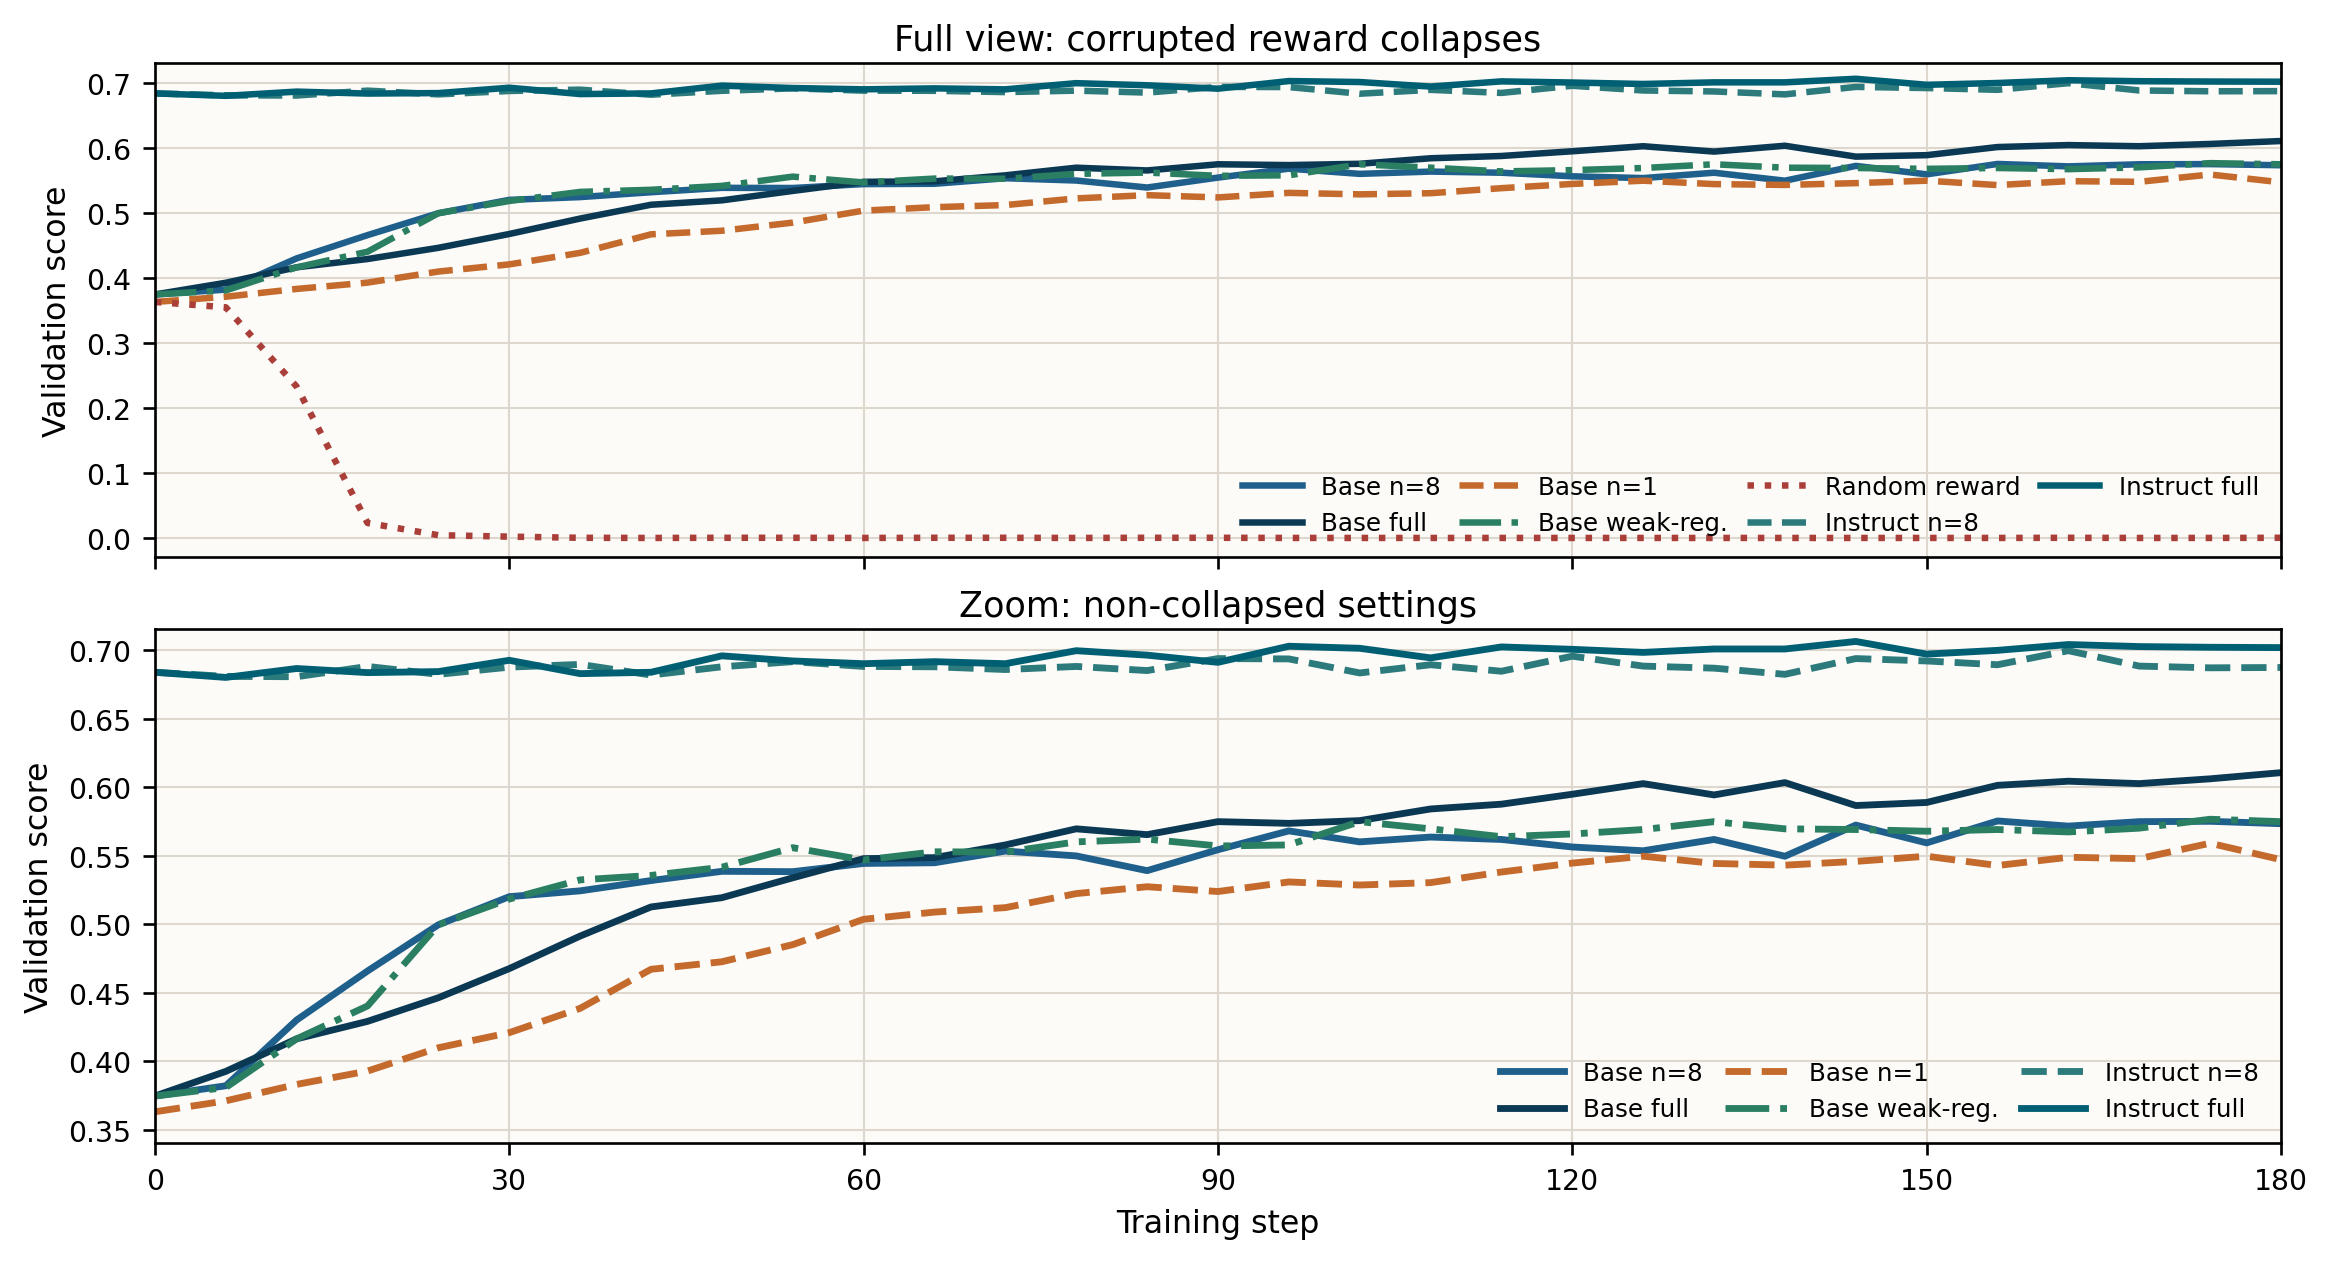
\includegraphics[width=\linewidth,height=0.72\textheight,keepaspectratio]{pic/score-main-seven-settings-with-zoom.png}
\end{figure}
\small Base 1-shot GRPO improves strongly; corrupted rewards collapse, so the effect is not generic RL.
\end{frame}

% 6
\begin{frame}[shrink=4]{Answer 1: The Gain Is Real but Conditional}
\scriptsize
\begin{table}
\centering
\resizebox{\textwidth}{!}{%
\begin{tabular}{lccc}
\toprule
\textbf{Setting} & \textbf{Best Acc.} & \textbf{Final Acc.} & \textbf{Role} \\
\midrule
Base n=8 & 0.603 & 0.583 & Main low-data result \\
Base full-data & 0.611 & 0.611 & Full-data Base reference \\
Base n=1 & 0.559 & 0.547 & Group-size ablation \\
Base weak-reg. & 0.577 & 0.575 & Regularization ablation \\
Base random-reward & 0.363 & 0.000 & Strict negative control \\
Instruct n=8 & 0.700 & 0.687 & 1-shot Instruct result \\
Instruct full-data & 0.706 & 0.702 & Full-data Instruct reference \\
\bottomrule
\end{tabular}
}
\end{table}

\takeaway{1-shot GRPO gives a substantial Base-model gain, but the gain depends on meaningful rewards and does not remove the value of full data.}
\end{frame}

% 7
\begin{frame}{Question 2: How Much Comes From Data Budget?}
\begin{columns}
\column{0.55\textwidth}
\begin{figure}
    \centering
    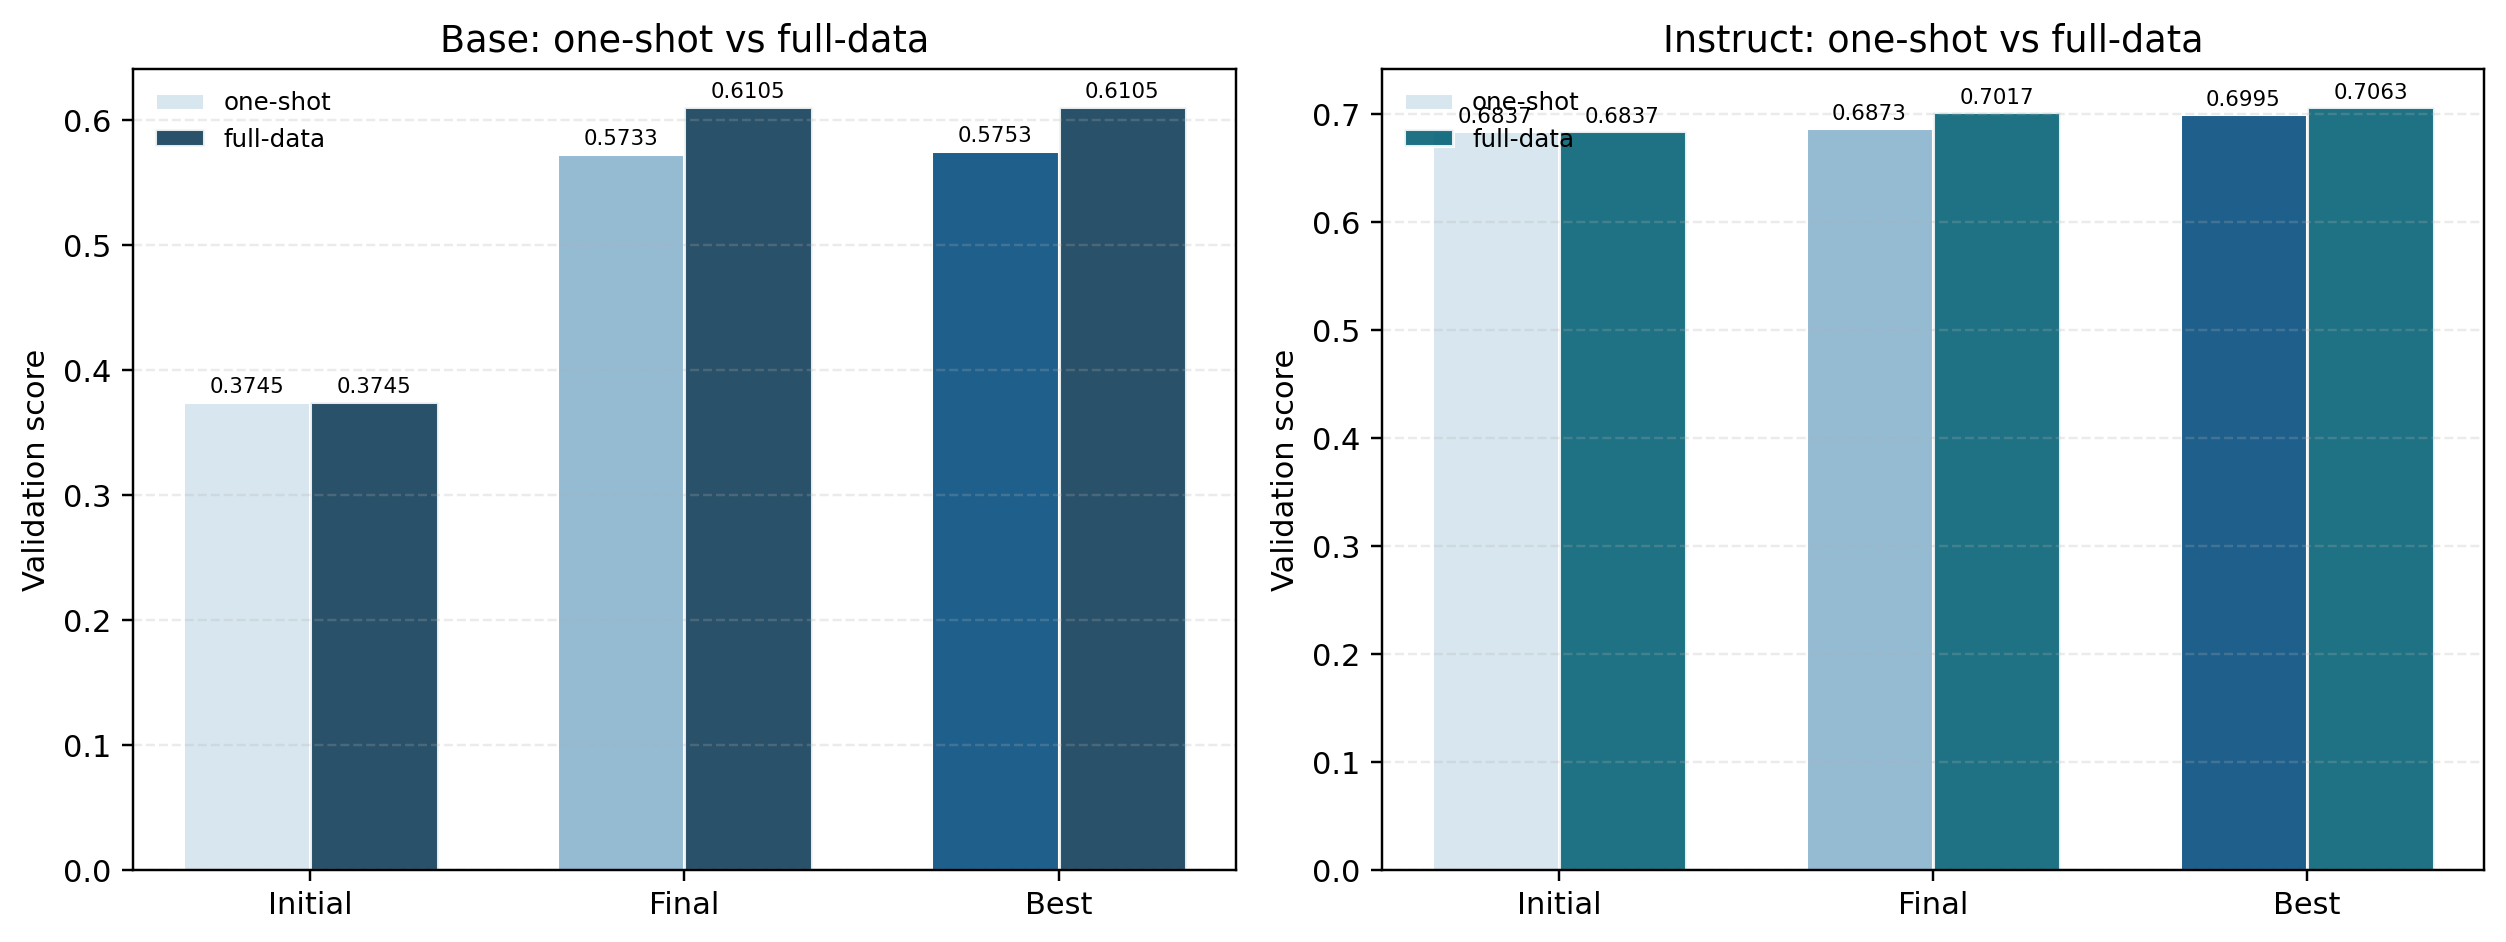
\includegraphics[width=\linewidth,height=0.58\textheight,keepaspectratio]{pic/matched-full-data-panel.png}
\end{figure}

\column{0.45\textwidth}
\begin{block}{Interpretation}
\begin{itemize}
    \item Base final gap: +0.0373 for full-data over one-shot.
    \item Instruct final gap: +0.0145.
    \item One-shot captures a clean low-data gain, but full-data still improves the endpoint.
\end{itemize}
\end{block}
\end{columns}
\end{frame}

% 8
\begin{frame}{Question 3: What Changes in the Output Distribution?}
\begin{figure}
    \centering
    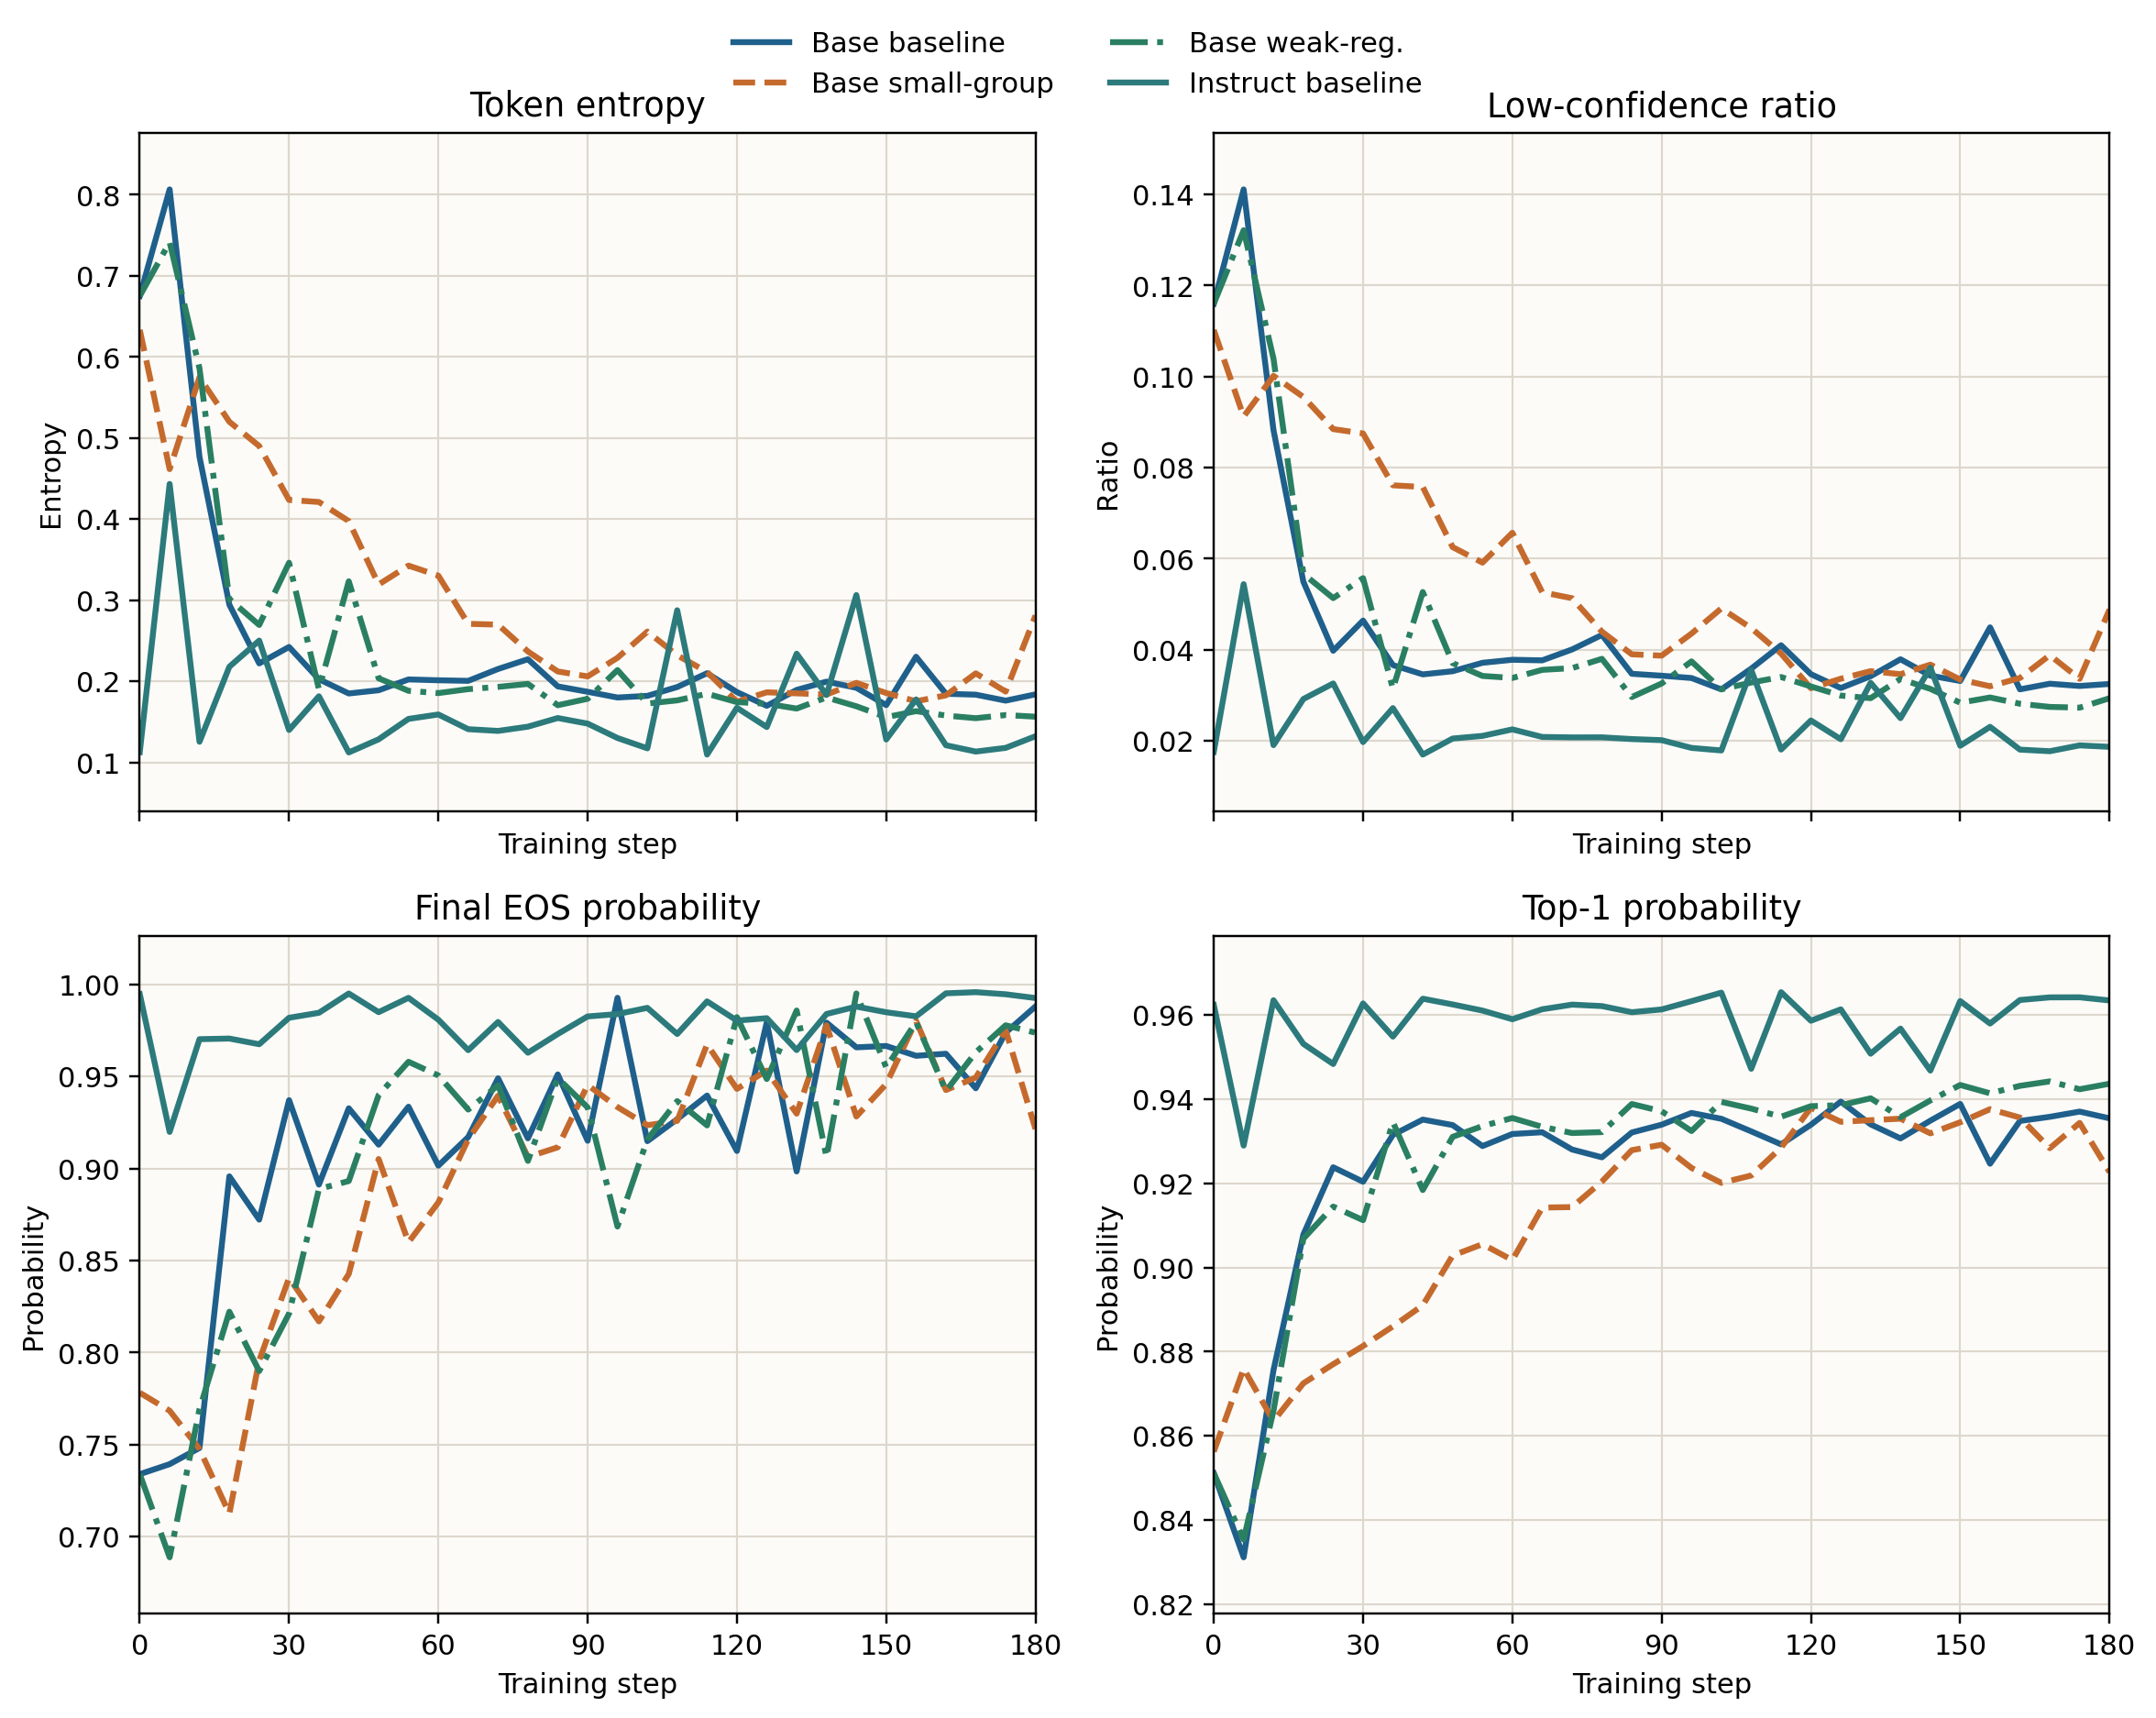
\includegraphics[width=\linewidth,height=0.60\textheight,keepaspectratio]{pic/behavior-detail-main-settings-panel.png}
    \caption{Length, entropy, top-1 probability, EOS probability, and tail confidence.}
\end{figure}
\small Successful settings move toward shorter, lower-entropy, higher-confidence generation.
\end{frame}

% 9
\begin{frame}{Mechanism Signal: Correct Responses Are Better Calibrated}
\begin{figure}
    \centering
    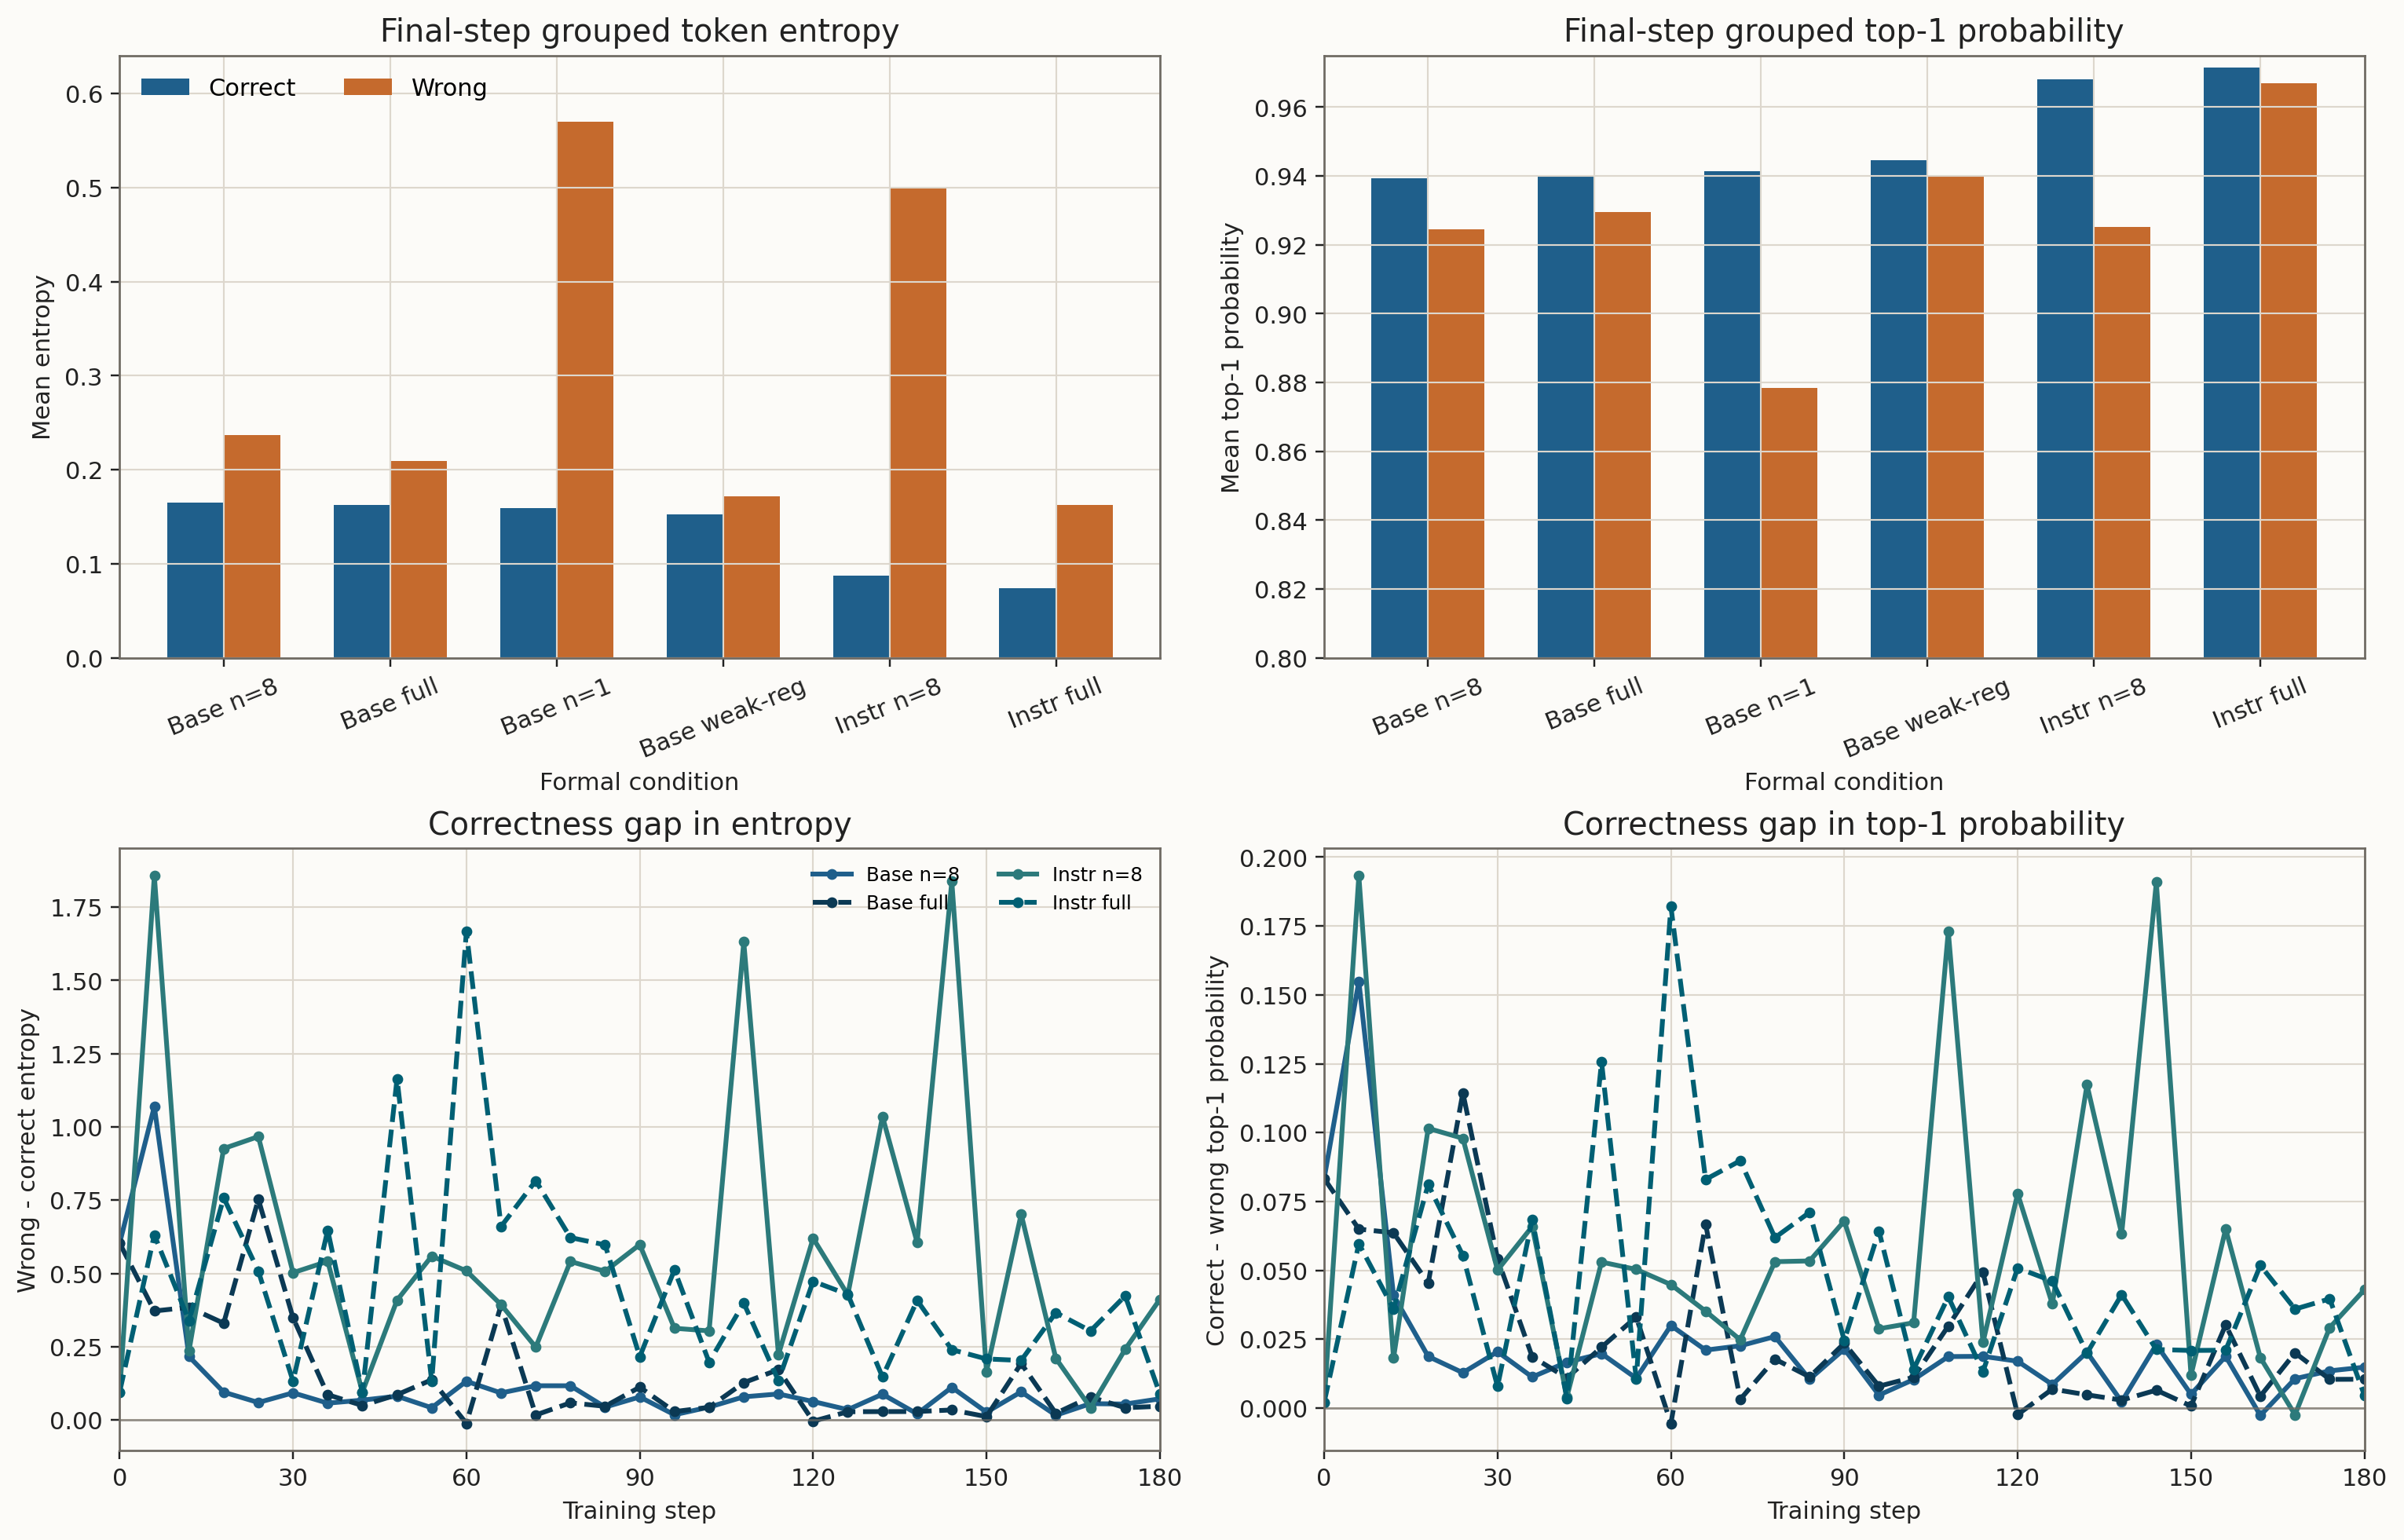
\includegraphics[width=\linewidth,height=0.60\textheight,keepaspectratio]{pic/correct-wrong-support-panel.png}
\end{figure}
\small Correct responses are systematically lower-entropy and higher-confidence than wrong responses across the non-collapse settings. This links score gains to distributional stabilization, not only endpoint accuracy.
\end{frame}

% 10
\begin{frame}[shrink=4]{Full-Token Audit: Testing the Mechanism Directly}
\small
\begin{block}{Protocol}
Base n=8 1-shot checkpoints at steps 0, 60, 120, 180; 32 held-out problems; 4 sampled responses per problem; every generated token is scored.
\end{block}

\begin{table}
\centering
\scriptsize
\begin{tabular}{rccccc}
\toprule
Step & Score & Len. & Ent. & Low-conf. & Top-1 \\
\midrule
0 & 0.305 & 812.1 & 0.698 & 0.125 & 0.839 \\
60 & 0.617 & 609.9 & 0.239 & 0.045 & 0.918 \\
120 & 0.586 & 608.9 & 0.271 & 0.049 & 0.915 \\
180 & 0.617 & 662.9 & 0.219 & 0.040 & 0.926 \\
\bottomrule
\end{tabular}
\end{table}

\takeaway{The main behavioral transition appears early: higher score, shorter responses, lower entropy, and fewer low-confidence tokens.}
\end{frame}

% 11
\begin{frame}{Mechanism Over Checkpoints}
\begin{figure}
    \centering
    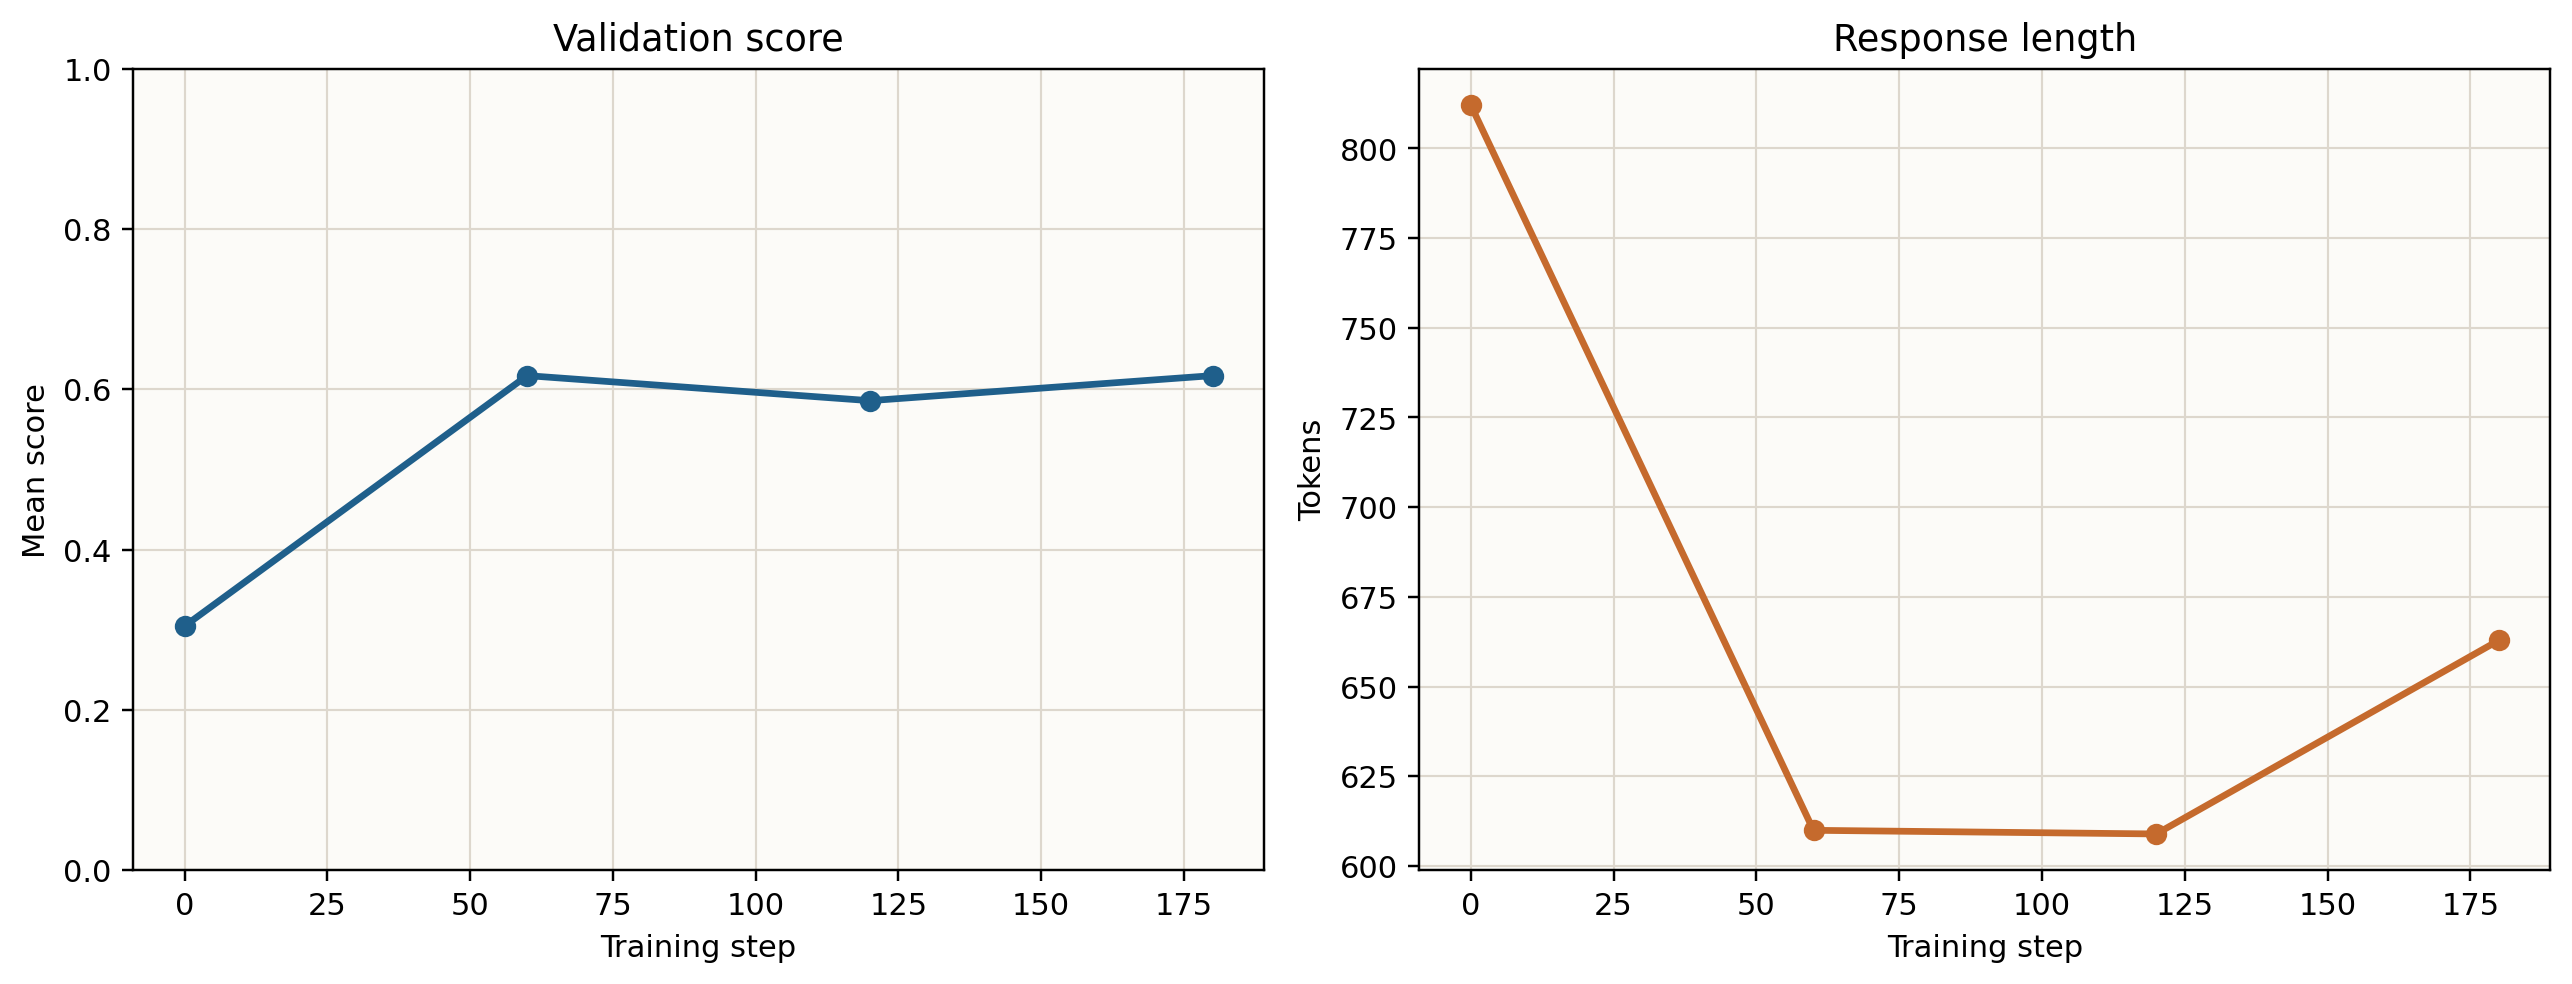
\includegraphics[width=\linewidth,height=0.32\textheight,keepaspectratio]{pic/full-token-score-length.png}
    \vspace{0.2em}
    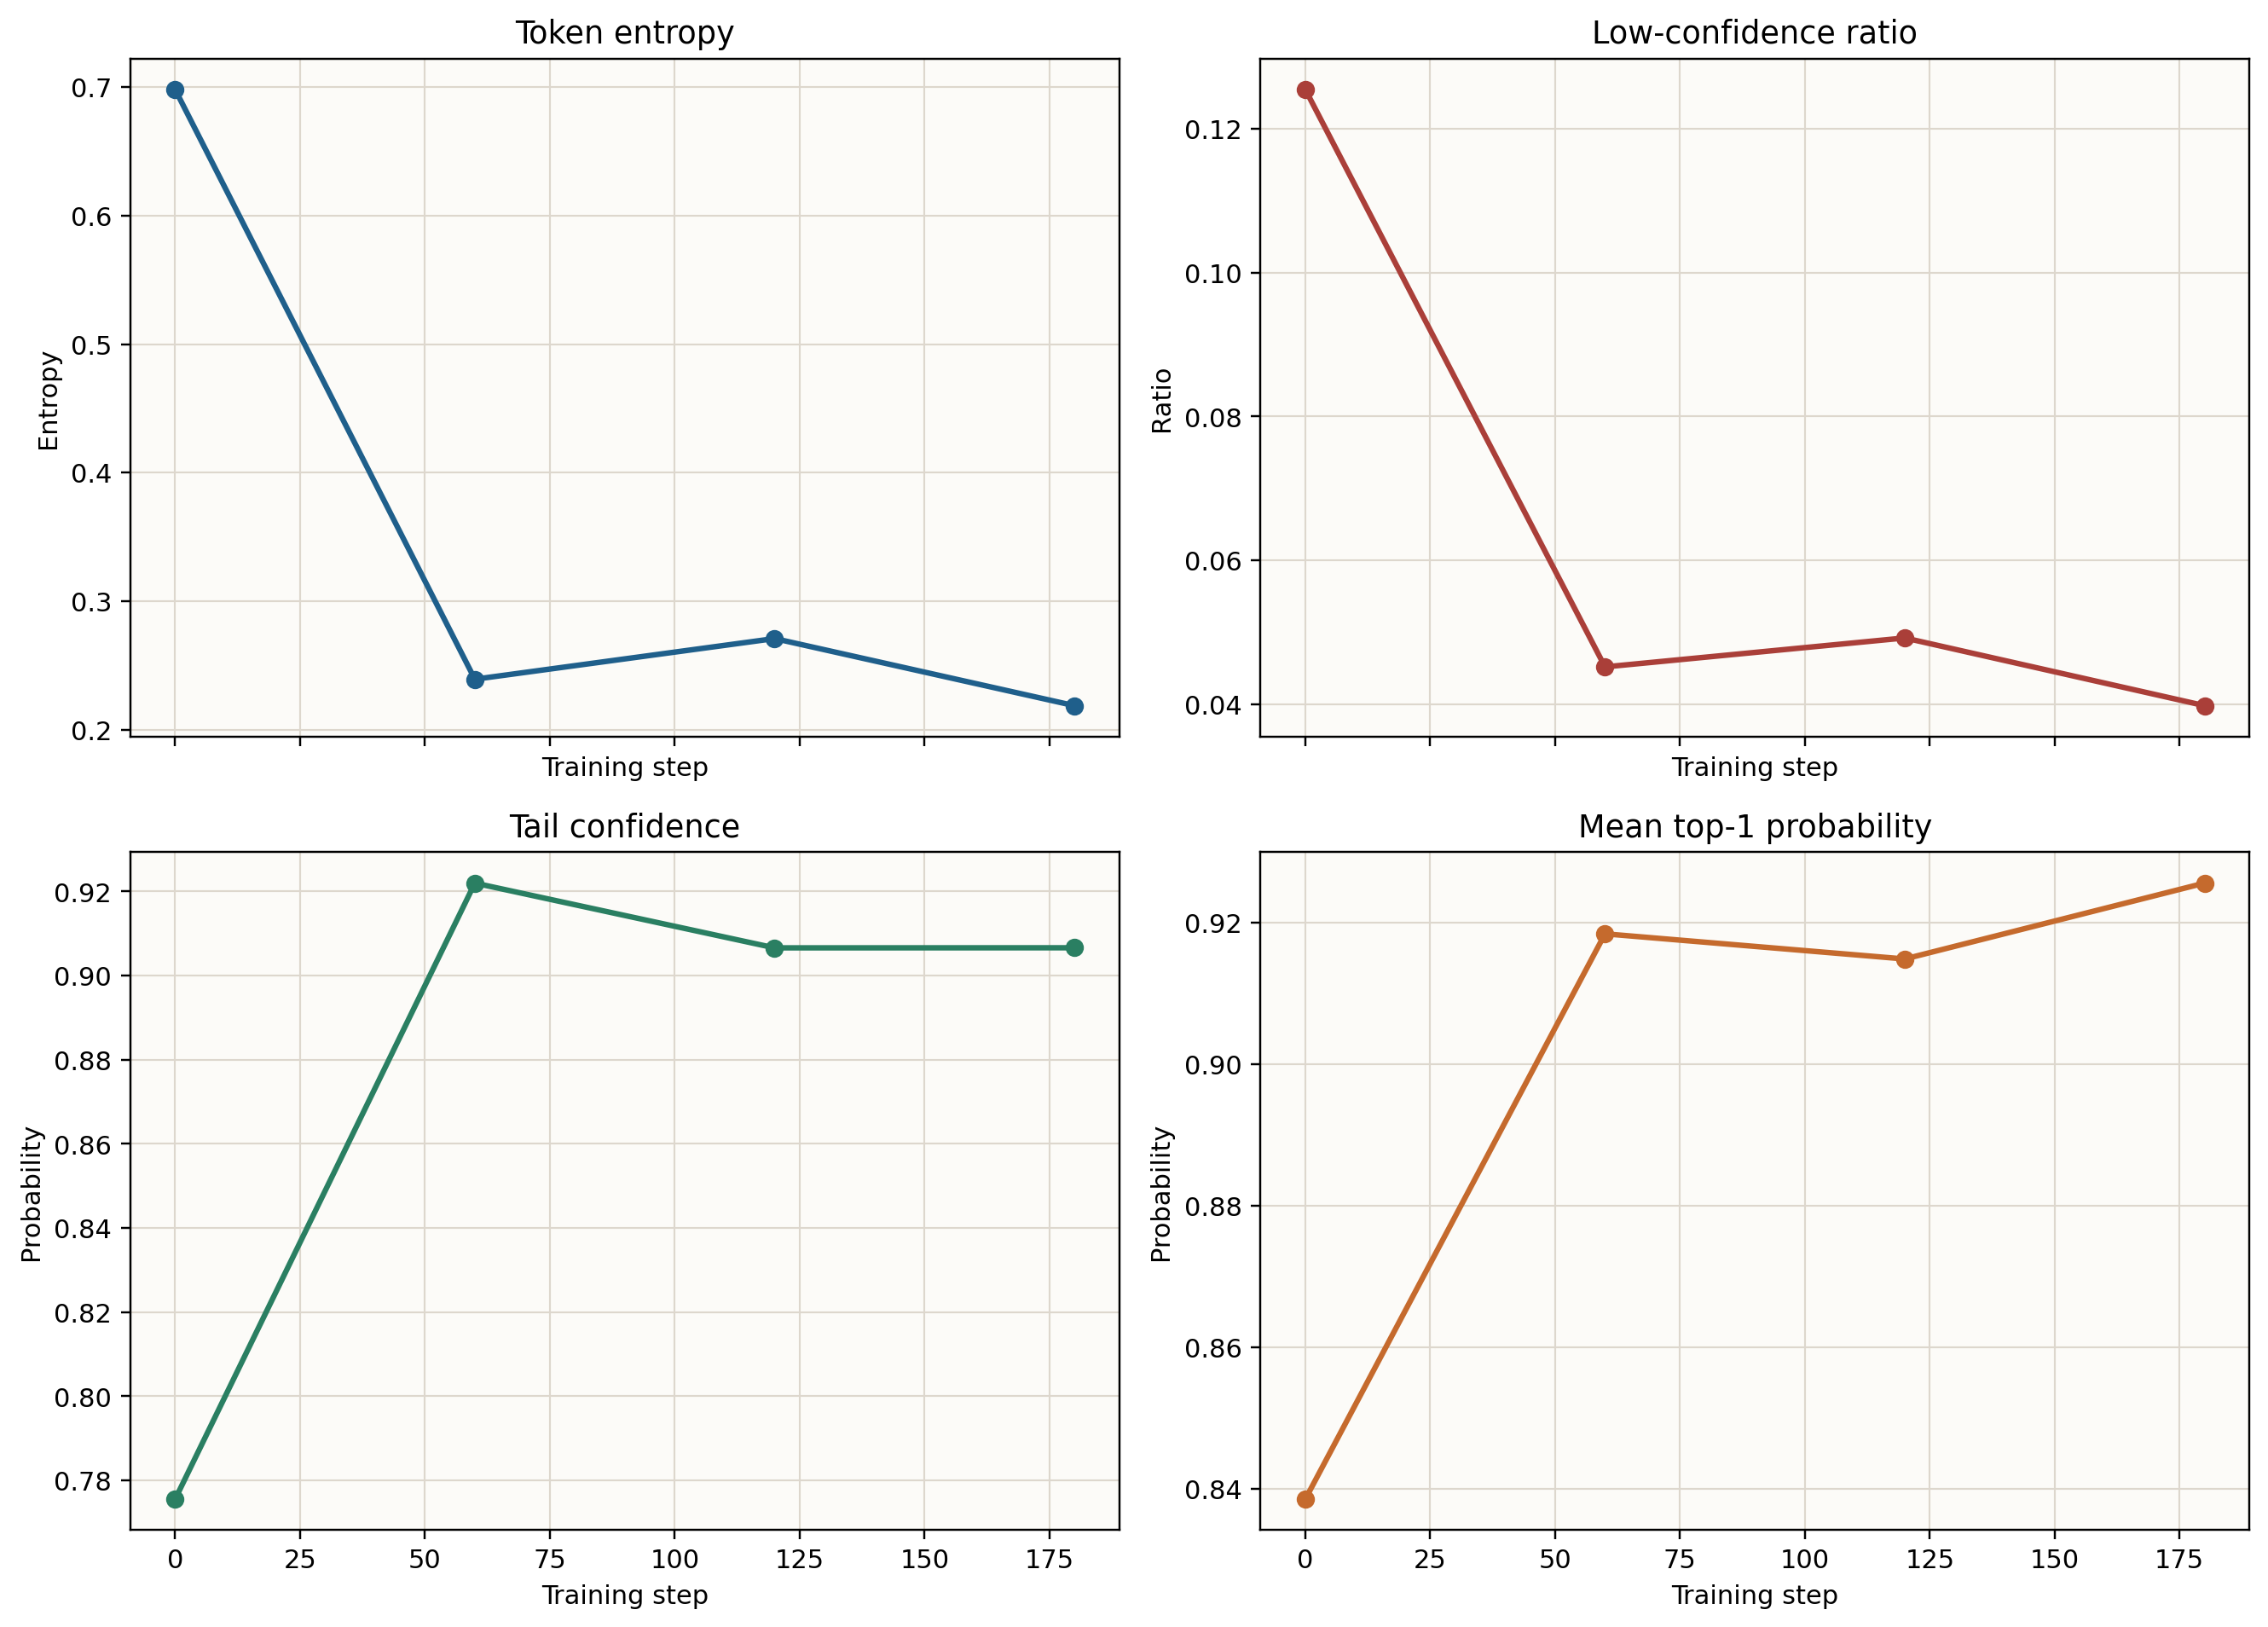
\includegraphics[width=\linewidth,height=0.30\textheight,keepaspectratio]{pic/full-token-confidence-panel.png}
\end{figure}
\small The main transition occurs by step 60: score rises while length, entropy, and low-confidence mass fall sharply. This looks like rapid calibration, not slow knowledge acquisition.
\end{frame}

% 12
{
\setbeamertemplate{navigation symbols}{}
\begin{frame}[plain]
\centering
\makebox[\textwidth][c]{%
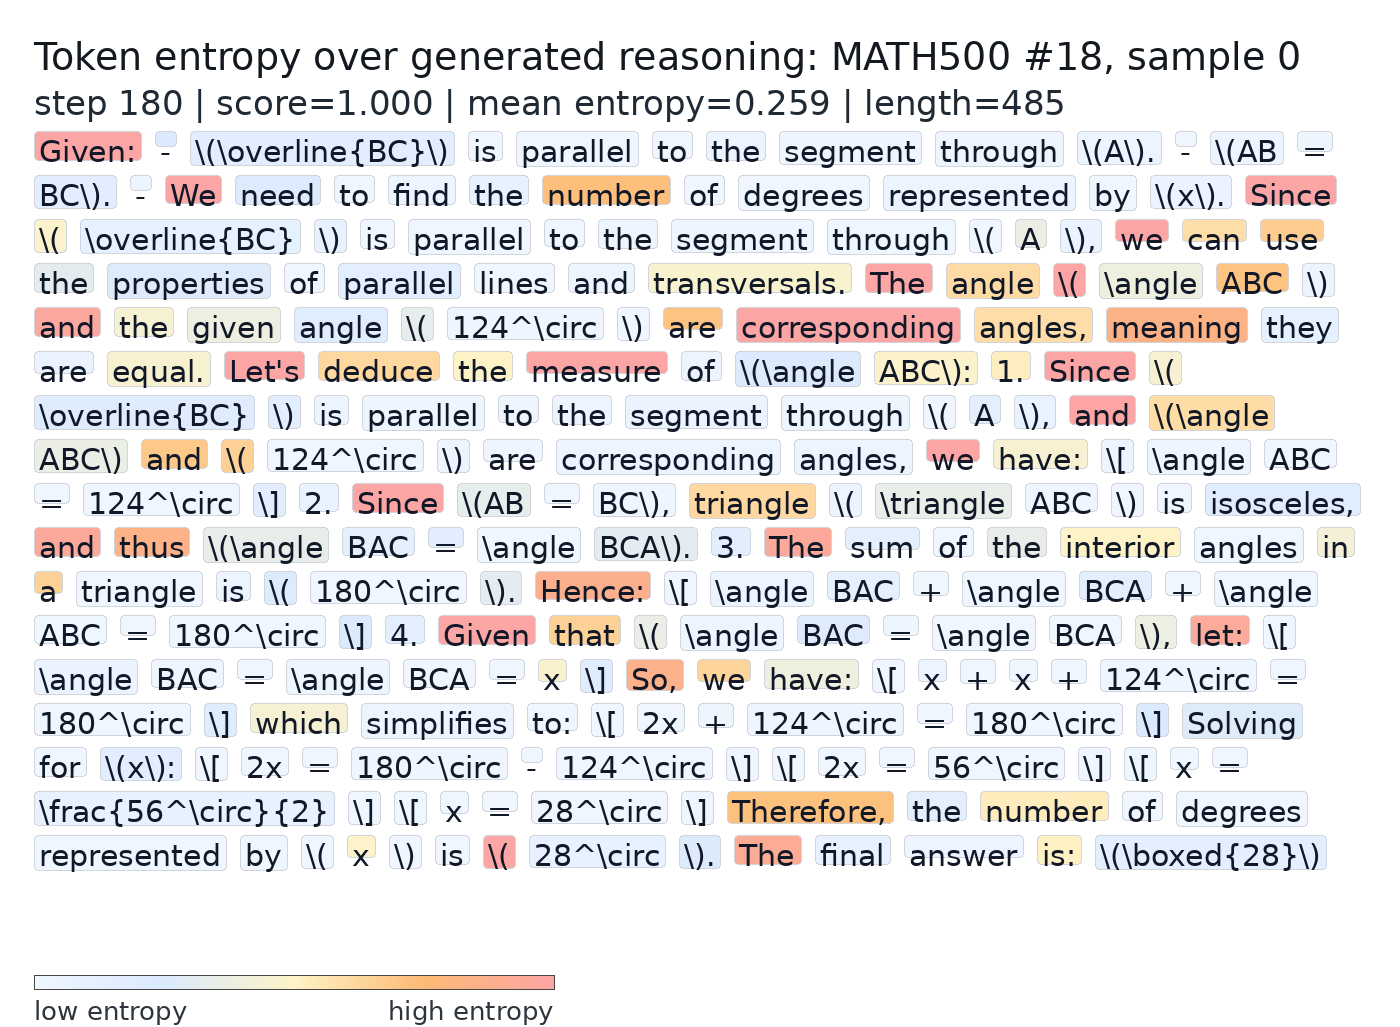
\includegraphics[width=0.98\paperwidth,height=0.96\paperheight,keepaspectratio]{pic/trajectory-text-entropy-score1-fullslide.png}%
}
\end{frame}
}

% 13
{
\setbeamertemplate{navigation symbols}{}
\begin{frame}[plain]
\centering
\makebox[\textwidth][c]{%
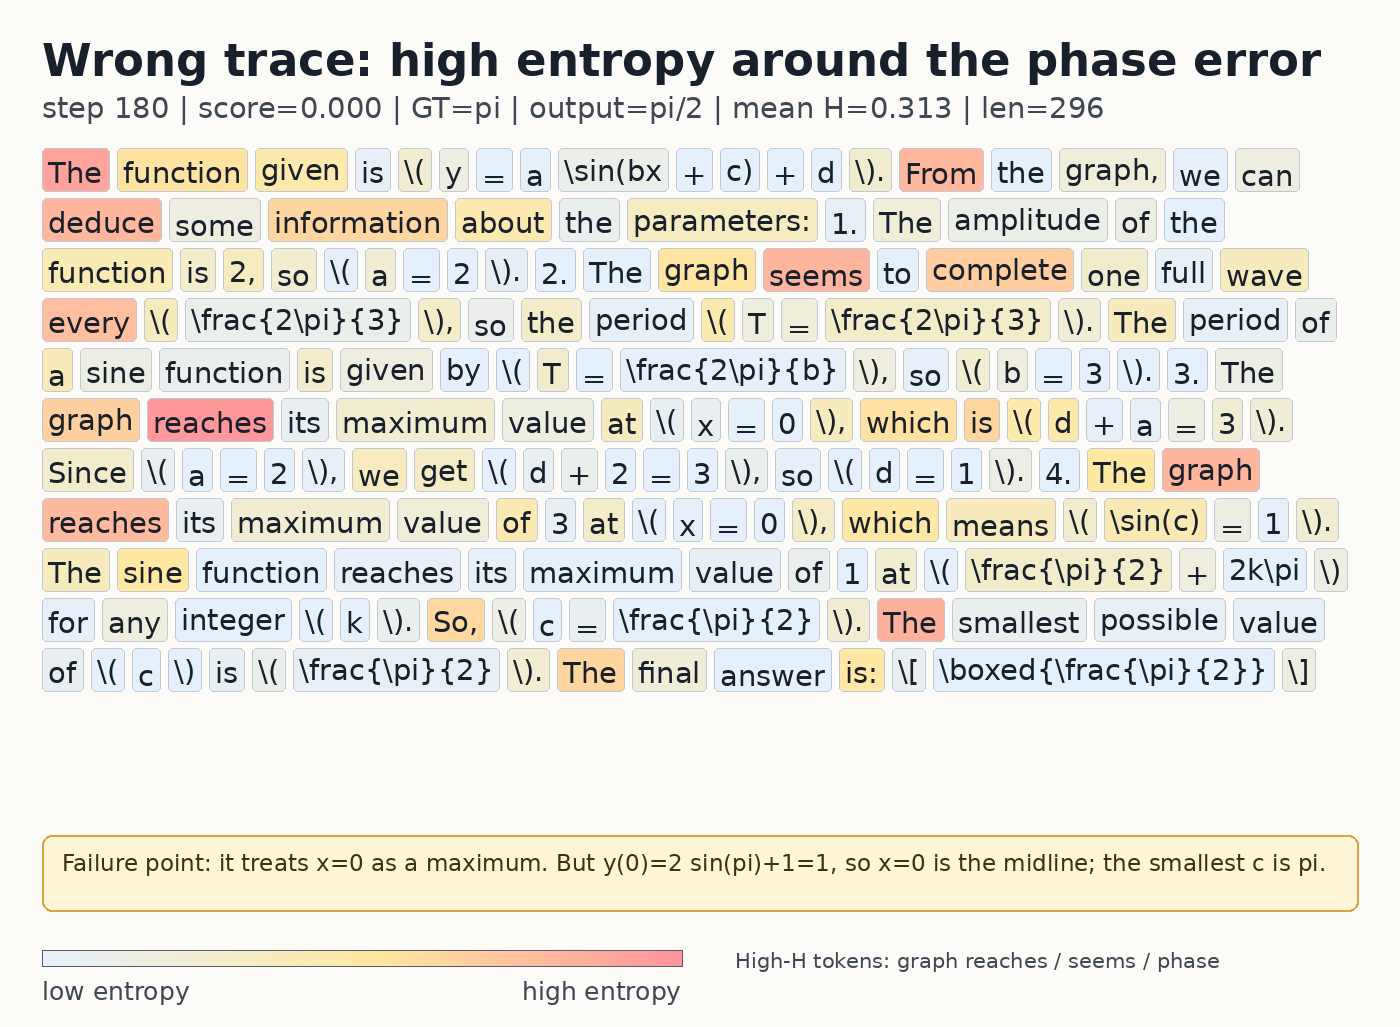
\includegraphics[width=0.98\paperwidth,height=0.96\paperheight,keepaspectratio]{pic/trajectory-text-entropy-wrong-sine-fullslide.png}%
}
\end{frame}
}

% 14
\begin{frame}{Mechanism Interpretation}
\begin{block}{Why the Gain Looks Like Calibration}
\begin{itemize}
    \item The gain is not produced by longer exploration: step 60 is much shorter than step 0.
    \item Step 60 and step 180 tie in score but differ behaviorally, so no single token metric explains everything.
    \item At the final checkpoint, correct responses remain lower-entropy, while wrong traces can reveal high-entropy mistaken premises.
    \item EOS pressure drops after training and only partly rebounds at step 180, so the gain is not just early stopping.
\end{itemize}
\end{block}

\takeaway{The mechanism is a coordinated shift in generation behavior: confidence, entropy, length, and stopping behavior move together.}
\end{frame}

% 15
\begin{frame}[shrink=6]{Source of the Gain: Reward Semantics Matter}
\begin{figure}
    \centering
    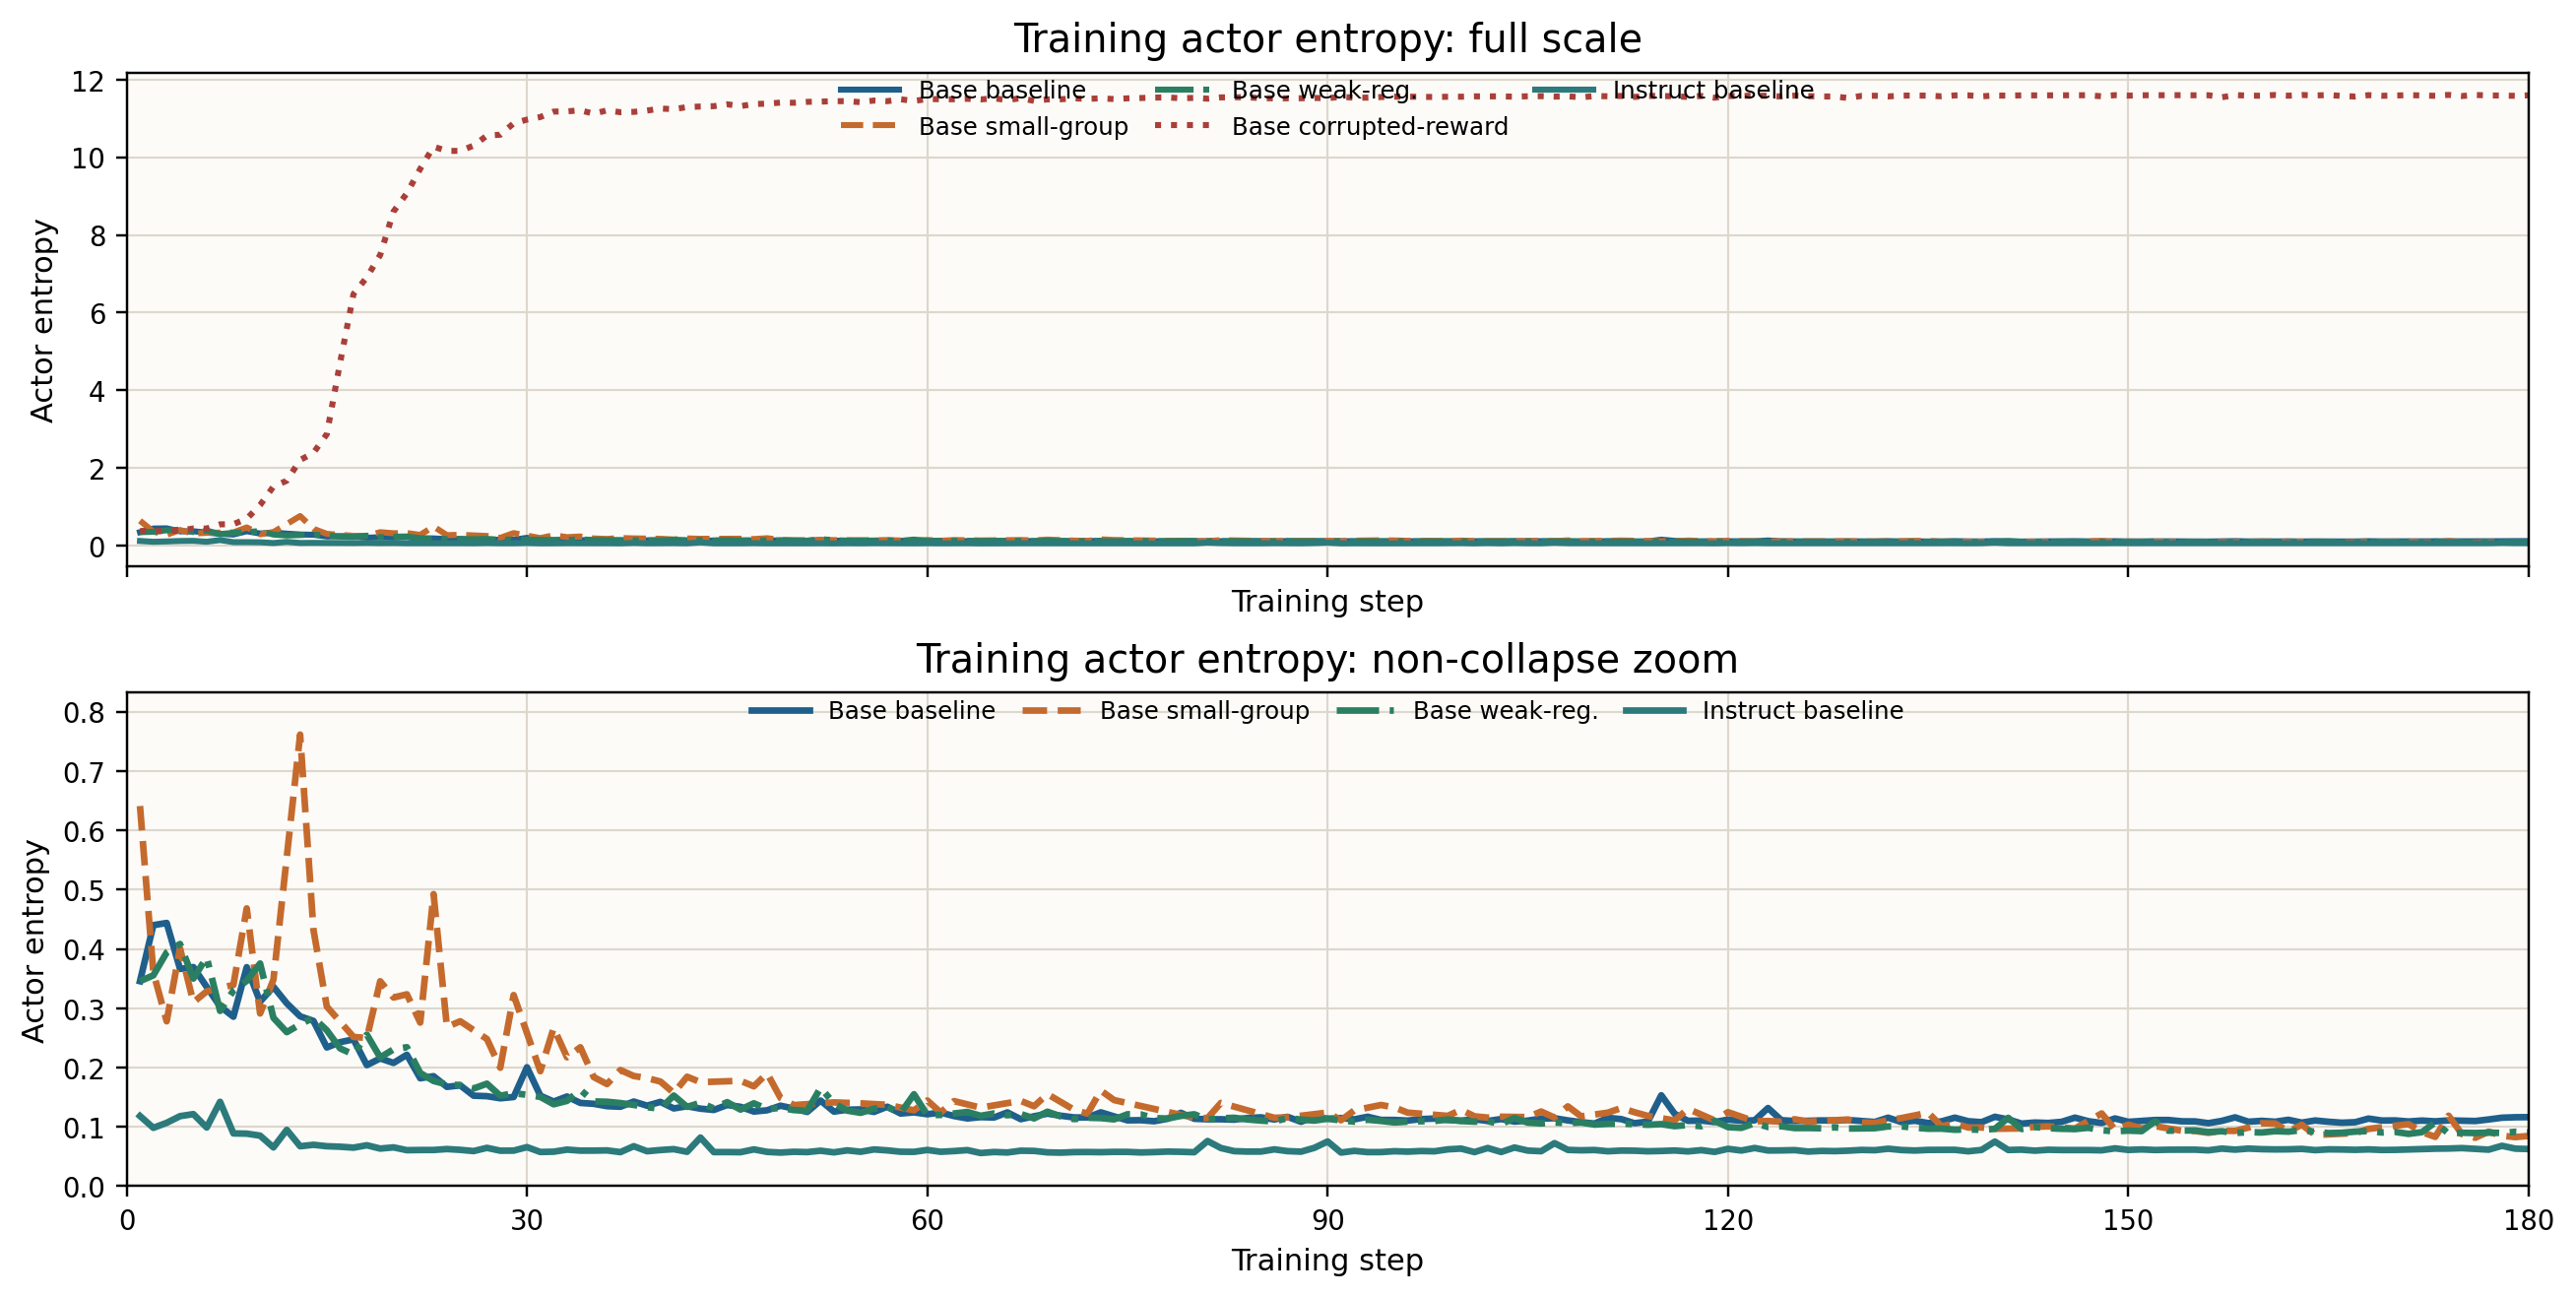
\includegraphics[width=\linewidth,height=0.70\textheight,keepaspectratio]{pic/actor-entropy-static-vertical.png}
\end{figure}

\vspace{-0.8em}
\begin{block}{Reading}
\scriptsize
\begin{itemize}
    \setlength{\itemsep}{0.15em}
    \item Successful runs reduce uncertainty without matching the corrupted-reward collapse.
    \item Random-reward training moves into an unstable distributional regime.
    \item Weak regularization remains competitive, so the story is not simply stronger entropy suppression.
\end{itemize}
\end{block}
\end{frame}

% 16
\begin{frame}{Answering the Three Questions}
\begin{block}{1. Does 1-shot GRPO have a benefit?}
Yes for the Base model: \texttt{Base n=8} reaches 0.603 best accuracy and 0.583 final accuracy.
\end{block}

\begin{block}{2. Where does the benefit come from?}
It depends on meaningful reward semantics and grouped rollout comparison; full-data still improves the endpoint, so one-shot is useful but not a complete substitute.
\end{block}

\begin{block}{3. What is the mechanism?}
The evidence points to behavioral calibration: shorter responses, lower entropy, higher top-1 probability, fewer low-confidence tokens, and trace-level entropy around reasoning choices.
\end{block}
\end{frame}

% 17
\begin{frame}{Thank You}
\begin{center}
    {\Huge Thank You} \\
\end{center}
\end{frame}

\end{document}
